\documentclass[12pt]{article}
\setlength\parindent{0pt}
\usepackage{fullpage}
\usepackage{graphicx}
\usepackage{amsmath}
\setlength{\parskip}{4mm}
\def\LL{\left\langle}   % left angle bracket
\def\RR{\right\rangle}  % right angle bracket
\def\LP{\left(}         % left parenthesis
\def\RP{\right)}        % right parenthesis
\def\LB{\left\{}        % left curly bracket
\def\RB{\right\}}       % right curly bracket
\def\PAR#1#2{ {{\partial #1}\over{\partial #2}} }
\def\PARTWO#1#2{ {{\partial^2 #1}\over{\partial #2}^2} }
\def\PARTWOMIX#1#2#3{ {{\partial^2 #1}\over{\partial #2 \partial #3}} }
\newcommand{\BE}{\begin{displaymath}}
\newcommand{\EE}{\end{displaymath}}
\newcommand{\BNE}{\begin{equation}}
\newcommand{\ENE}{\end{equation}}
\newcommand{\BEA}{\begin{eqnarray}}
\newcommand{\EEA}{\nonumber\end{eqnarray}}
\newcommand{\EL}{\nonumber\\}
\newcommand{\la}[1]{\label{#1}}
\newcommand{\ie}{{\em i.e.\ }}
\newcommand{\eg}{{\em e.\,g.\ }}
\newcommand{\cf}{cf.\ }
\newcommand{\etc}{etc.\ }
\newcommand{\Tr}{{\rm tr}}
\newcommand{\etal}{{\it et al.}}
\newcommand{\OL}[1]{\overline{#1}\ } % overline
\newcommand{\OLL}[1]{\overline{\overline{#1}}\ } % double overline
\newcommand{\OON}{\frac{1}{N}} % "one over N"
\newcommand{\OOX}[1]{\frac{1}{#1}} % "one over X"



\begin{document}
\Large
\centerline{\sc{Homework 7}}
\normalsize
\centerline{\sc{Due Wednesday, 12 April}}

\begin{enumerate}

\item{In the classic computer game {\it Portal}, the player is asked to solve 
puzzles with the use of a ``portal device'', which can create two connected portals
on, for example, the floor and a wall. An object entering one portal with speed $v$
will exit the other with the same speed. Here's an illustration:

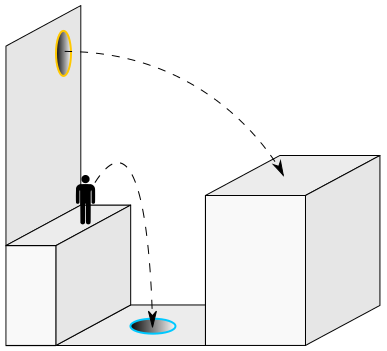
\includegraphics[width=0.4\textwidth]{Portal_physics-2.png}

The game's narrator helpfully explains that ``Forward momentum, a product of mass
and velocity, is conserved between portals. In layman's terms: {\bf speedy thing 
goes in; speedy thing comes out.}''
}
\begin{enumerate}
\item{Is this an accurate statement of the law of conservation of momentum? As the
narrator claims, does such a device conserve momentum? If not, why not?}
\item{Does this device conserve kinetic energy?}
\item{Does it conserve total energy (that is, kinetic energy $\frac{1}{2}mv^2$ 
plus gravitational potential energy $mgy$?}
\end{enumerate}

\item{A bowling ball (solid sphere; $I=\frac{2}{5}mr^2$) rolls down a hill
of height 5 meters. How fast is it traveling when it reaches the bottom?}

  \item{Knight 12.71 (3rd edition), reproduced below.}
  
    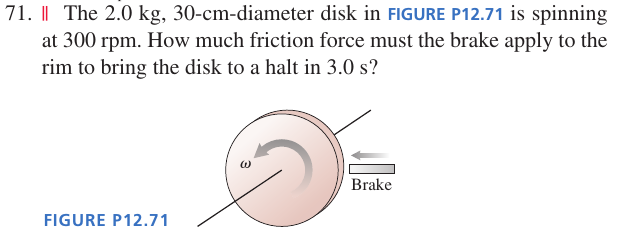
\includegraphics[width=0.6\textwidth]{brake.png}

  \item{Knight 12.31 (3rd edition), reproduced below.}
  
    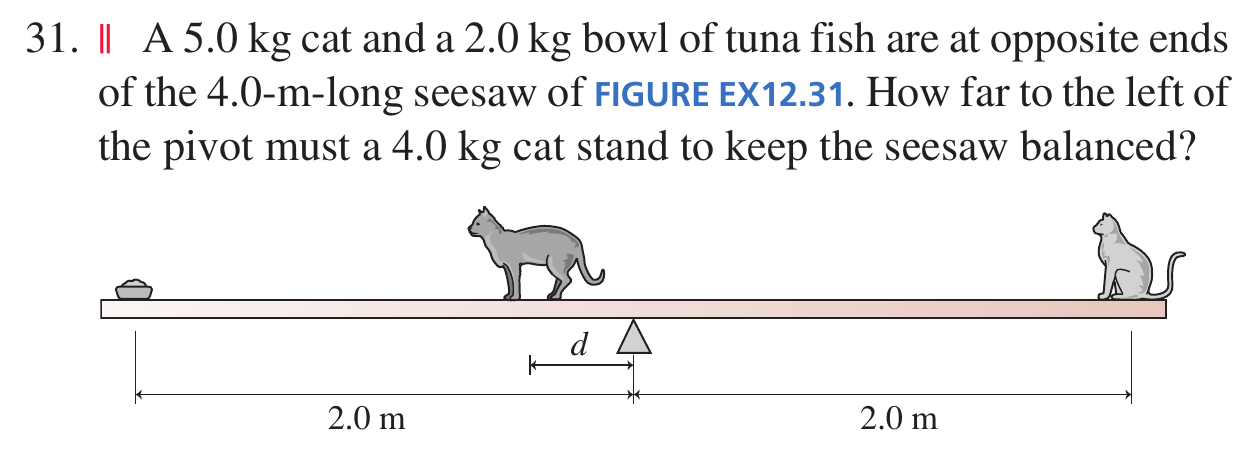
\includegraphics[width=0.6\textwidth]{cat.png}

  \item{Knight 12.63 (3rd edition), reproduced below. Note that normal forces can only push, not pull...}
  
    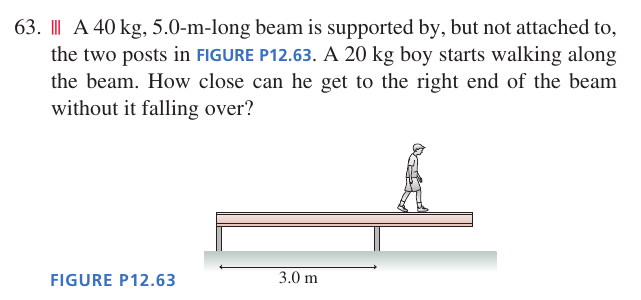
\includegraphics[width=0.6\textwidth]{torque2.png}

   \item{A bicyclist is riding a bicycle at a constant speed of 7 m/s. She has to pedal to overcome a drag force of 40 N. The bicycle's rear tire has a radius of 40 cm. There are two rear sprockets: one with a 
     radius of 5 cm (``high gear''), and one with a radius of 10 cm (``low gear''). The front sprocket has a radius of 10 cm. Note that the chain connecting the sprockets moves at a constant speed and thus has $a=0$, so the force it exerts on the front sprocket
   is the same as the force it exerts on the rear sprocket. {\em Note: The rotational equivalent to the power-velocity relation $P=\vec F \cdot \vec v$ is exactly what you think it would be: $P=\tau \omega$.}}

     \begin{enumerate}
       \item{When in high gear, how much torque must she deliver to the pedals to maintain her speed? What is her power output when doing so?}
       \item{When in low gear, how much torque must she deliver to the pedals to maintain her speed? What is her power output when doing so?}
       \item{Do your answers match your experience with riding a bicycle?}
     \end{enumerate}


\item {\it (This problem is worth ten points extra credit if you complete it fully.)}

A cylinder ($I=\frac{1}{2}mr^2$) rolls without slipping down an inclined plane of length $L$, angled at an angle $\theta$ to the horizontal. The 
coefficient of static friction between them is $\mu_s=0.5$.

\begin{enumerate}

\item Draw a (large) extended force diagram for the cylinder. Consider carefully in which direction the frictional force at the point of contact points. 
\item Is the frictional force equal to $\mu_s F_N$, or some other value that depends on the angle $\theta$? Explain, thinking about what happens as $\theta \rightarrow 0$.
(If the frictional force is not equal to $\mu_s F_N$, just use $F_f$ to represent it in equations.)
\item The ordinary ``translational'' work-energy theorem says that a force $\vec F$ acting over a displacement $\vec d$ causes a change in translational kinetic energy:
$\Delta (\frac{1}{2}mv^2) = \vec F \cdot \vec d$.
Find the ``translational work'' done by the gravitational force and by the frictional force.
\item The ``rotational'' work-energy theorem says that a torque $\tau $ acting over an object rotating through an angle $\Delta \theta$ causes a change in rotational kinetic energy: $\Delta (\frac{1}{2}I\omega^2) = \tau \Delta \theta$. 
Find the ``rotational work'' done by the gravitational force and by the frictional force.
\item If we consider ``translational kinetic energy'' $\frac{1}{2}mv^2$ and ``rotational kinetic energy'' $\frac{1}{2}I\omega^2$ as the same thing, what is the total
work (rotational plus translational) done by the frictional force?
\item Is it accurate to say that the frictional force here converts translational kinetic energy into rotational kinetic energy? Explain.
\item Comment on the validity of using energy methods to solve problems like (2). Do you need to worry about the frictional forces when considering translational
and rotational kinetic energy together?
\item By any method you like, calculate the size of the frictional force $F_f$. (There are two ways to do this. One involves energy methods; the other involves
examining the force diagram and thinking about the relation between $a$ and $\alpha$.)
\end{enumerate}
\end{enumerate}
    
    \end{document}
